\section*{Aufgabe 1}
\subsection*{Mittelwerte}

Die Mittelwerte der drei Populationen 
\begin{equation}
  \mu_\text{P1} = \begin{pmatrix} 5.99 \\ 2.98 \end{pmatrix} \text{ , } \mu_{P-0-10000} = \begin{pmatrix} 0.03 \\ 3.02 \end{pmatrix} \text{ und } \mu_{P-0-10000} = \begin{pmatrix} 0.03 \\ 3.02 \end{pmatrix}
\end{equation}
\subsection*{Kovarianzmatrizen}
Die Summierten Kovarianzmatrizen sind
\begin{equation}
  S^{P0} = \begin{pmatrix} 854102.52 & 569663.62 \\ 569663.62 & 470056.66 \end{pmatrix} \text{ und } S^{P1} = \begin{pmatrix} 122344.00 & 73117.72 \\ 73117.72 & 53984.57 \end{pmatrix}
\end{equation}
Die Summierte Kovarianzmatrix hat die From
\begin{equation}
  S^{P01,P00} = \begin{pmatrix} 976446.53 & 642781.33 \\ 642781.33 & 524041.22 \end{pmatrix}
\end{equation}
\subsection*{Fisher-Diskriiminante}
Die Fisherdiskrimante $\lambda$ beträgt 
\begin{equation}
  \lambda = \begin{pmatrix} -0.63 \\ 0.78 \end{pmatrix}
\end{equation}
Die Gradengleichung ergibt sich somit zu
\begin{equation}
  f(x) = -1.23 \cdot x \text{    bzw    } x_i = \lambda^T \vec{x}_i
\end{equation}
\subsection*{Population}
\begin{figure}[H]
  \centering
  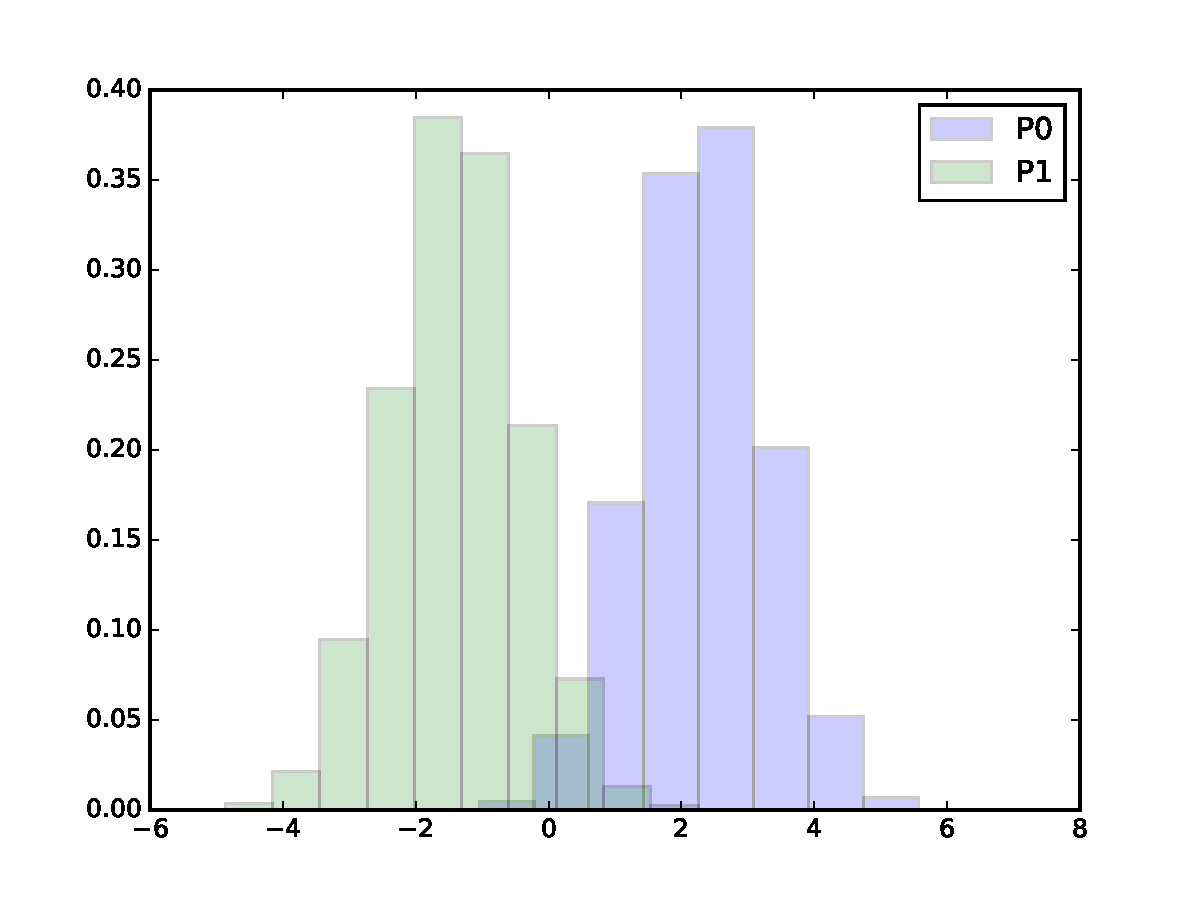
\includegraphics[height=7cm]{./Figures/firstHist.pdf}
  \caption{Abbildung der Populstionen auf die Grade}
\end{figure}
\subsection*{Reinheit}
\begin{figure}[H]
  \centering
  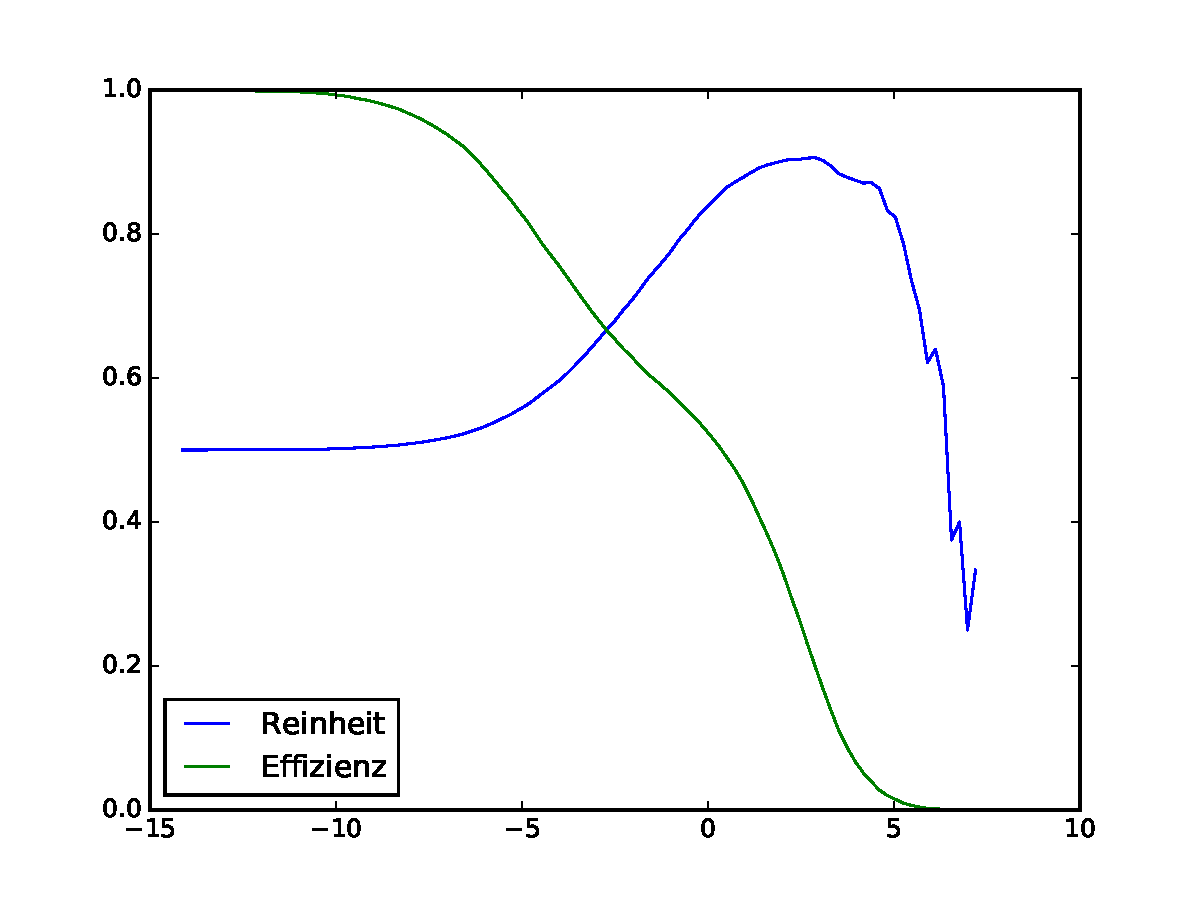
\includegraphics[height=7cm]{./Figures/reinheit1.pdf}
  \caption{Reinheit in Abhängigkeit des Schnittes}
\end{figure}
\subsection*{Signal zu Untergrundverhältnis}
\begin{figure}[H]
  \centering
  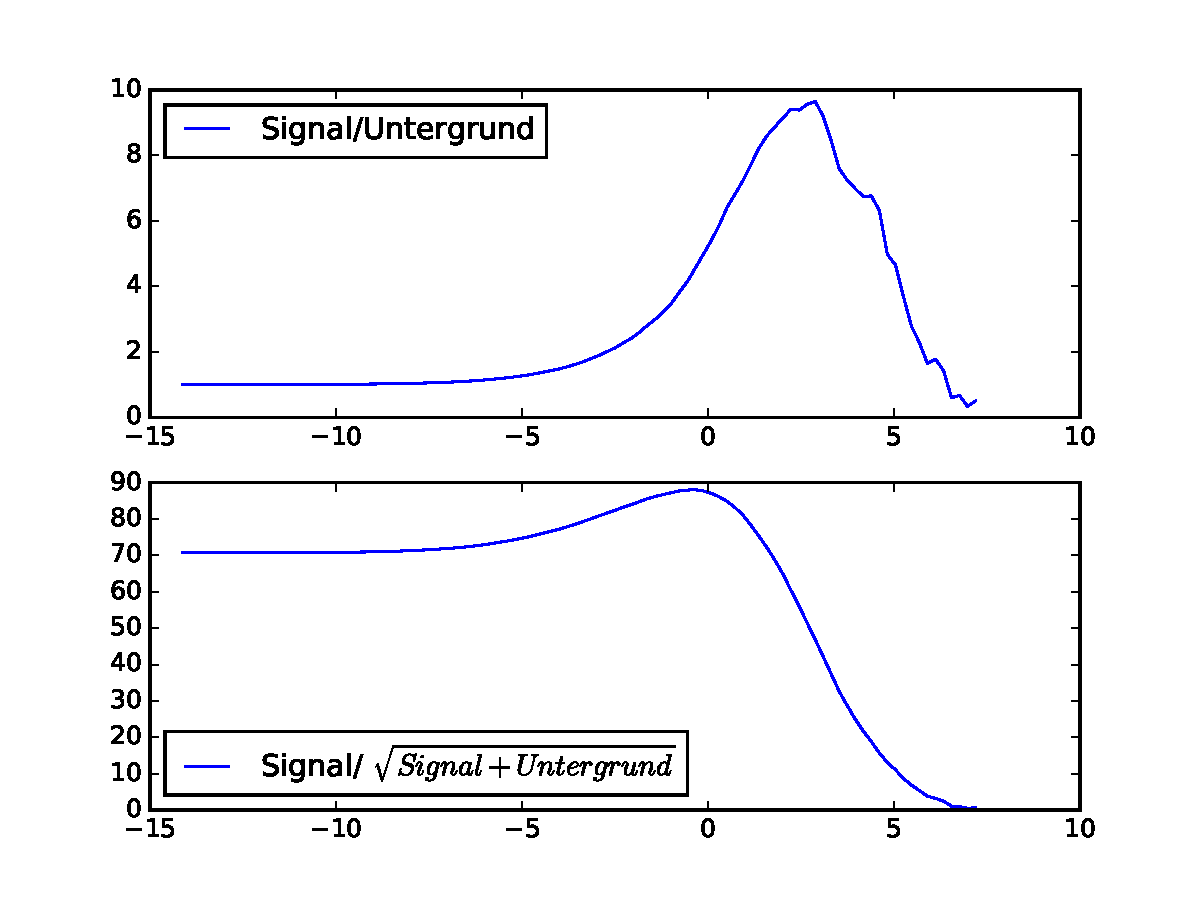
\includegraphics[height=7cm]{./Figures/SigZuUnt1.pdf}
  \caption{Signal zu Untergrundverhältnis sowie Signifikanz}
\end{figure}

\subsection*{Für die andere Population}

\begin{figure}[H]
  \centering
  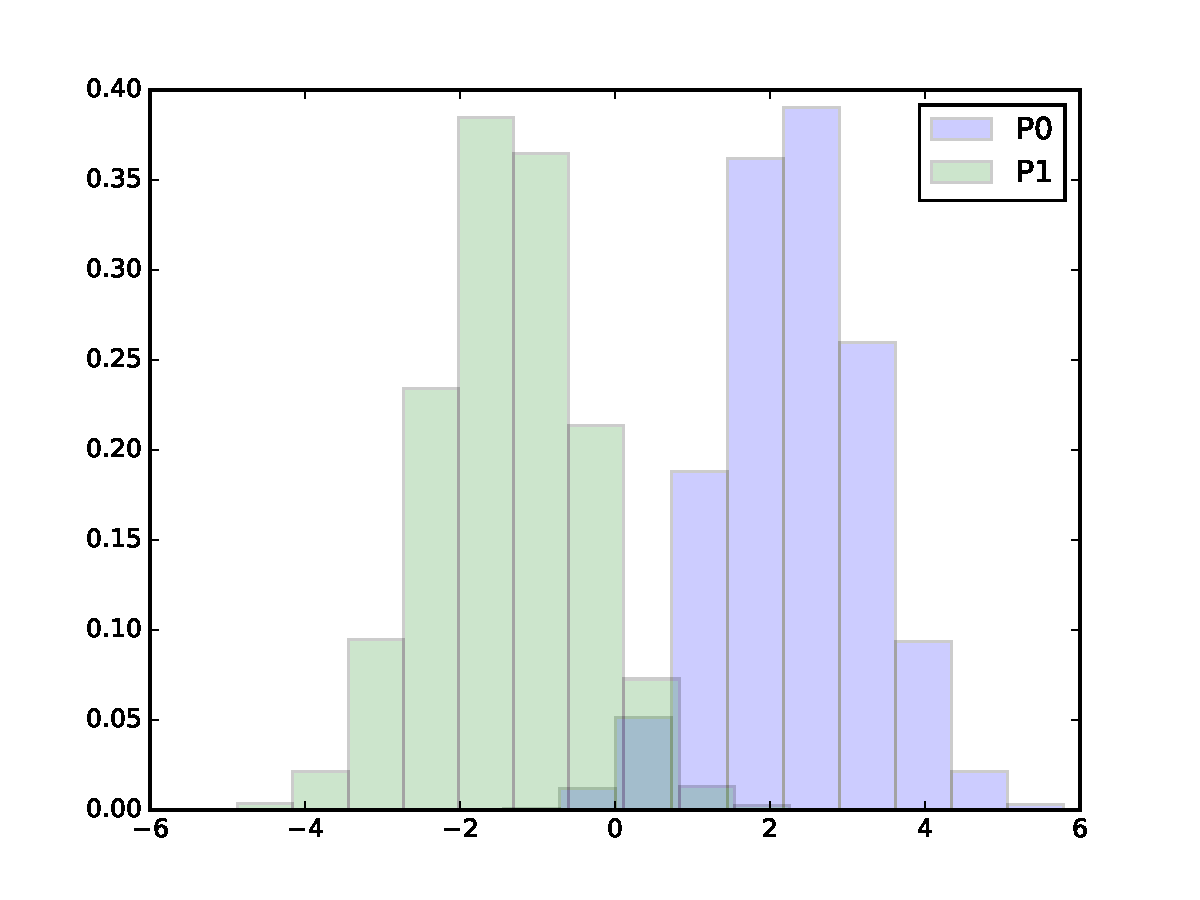
\includegraphics[height=7cm]{./Figures/secondHist.pdf}
  \caption{Abbildung der Populstionen auf die Grade}
\end{figure}

\begin{figure}[H]
  \centering
  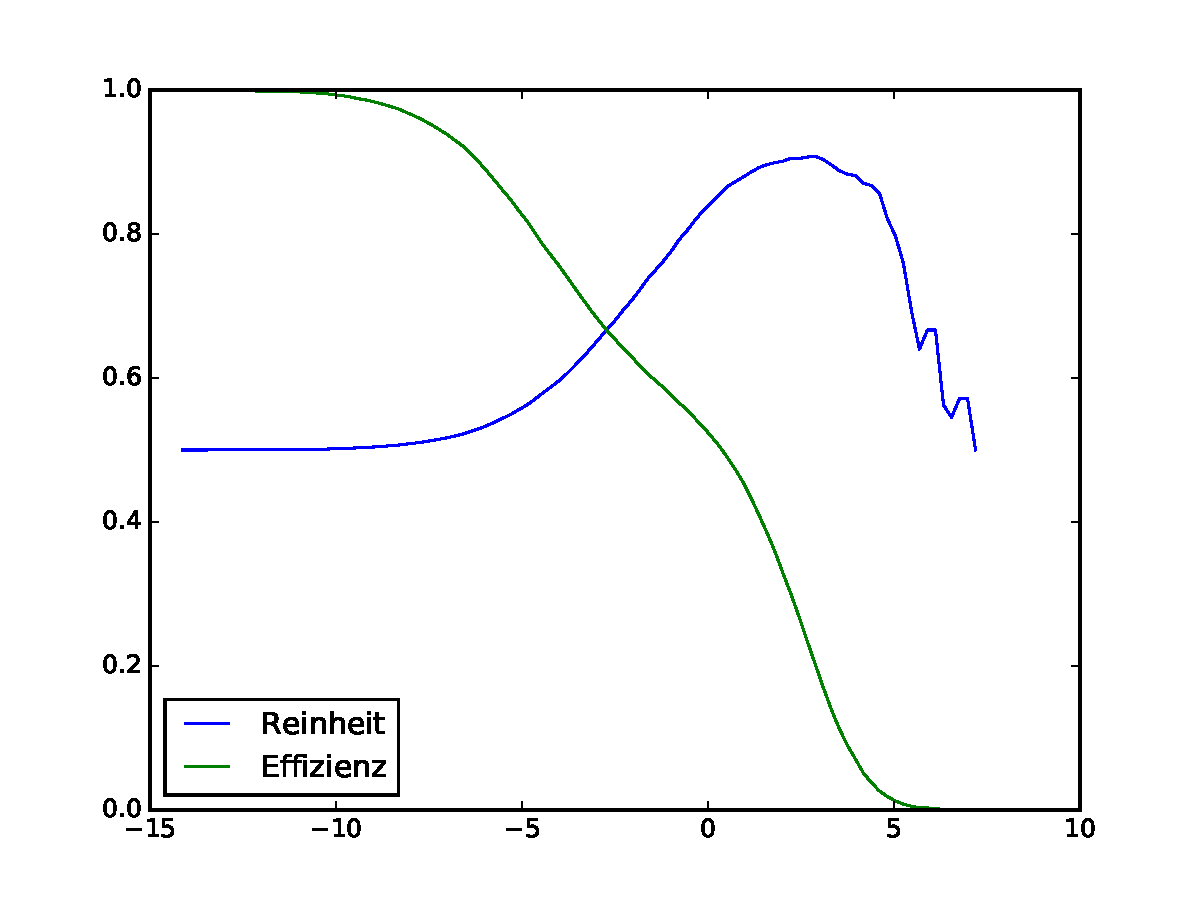
\includegraphics[height=7cm]{./Figures/reinheit2.pdf}
  \caption{Reinheit in Abhängigkeit des Schnittes}
\end{figure}

\begin{figure}[H]
  \centering
  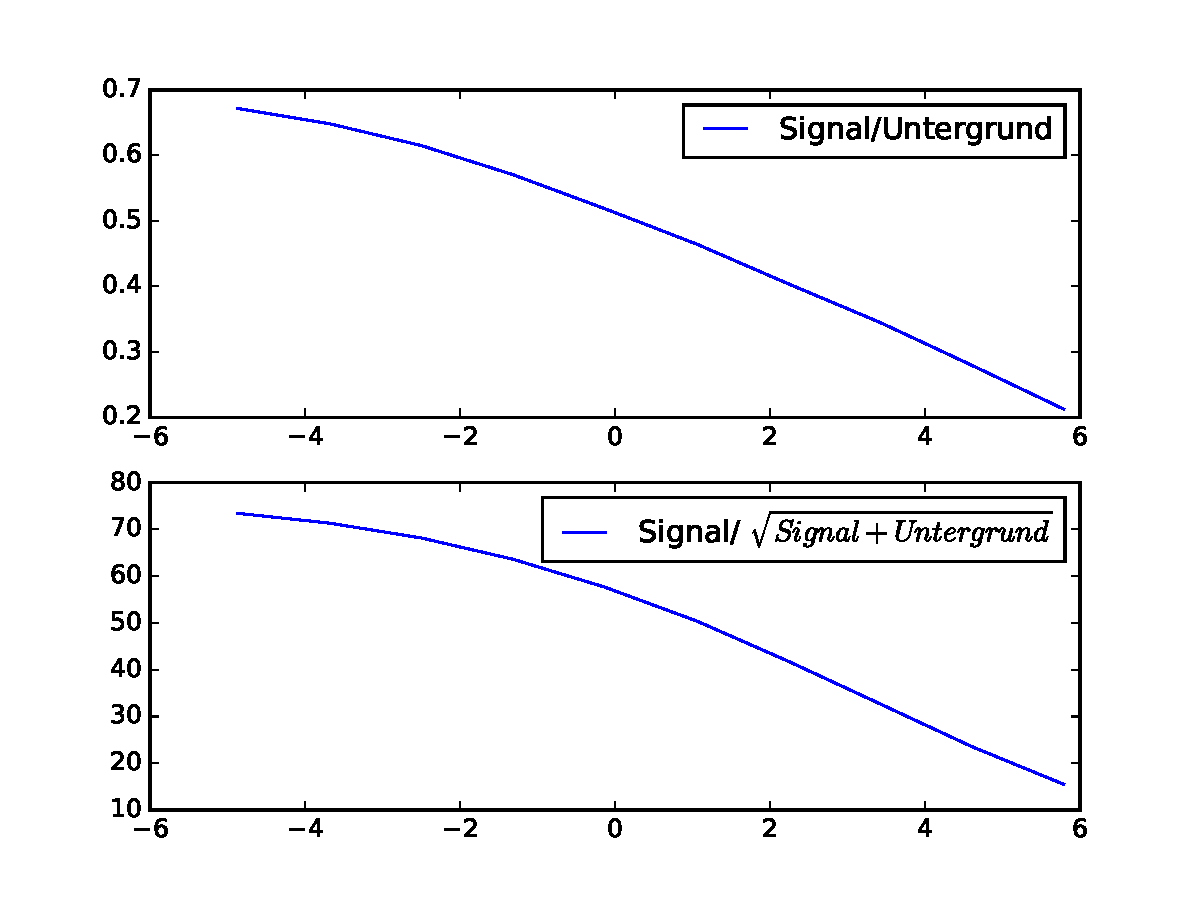
\includegraphics[height=7cm]{./Figures/SigZuUnt2.pdf}
  \caption{Signal zu Untergrundverhältnis sowie Signifikanz}
\end{figure}
